\section{Results}
\label{sec:results}

\subsection{Structured Tasks Saturate at a Single Schema Layer}
\label{sec:result-curves}

We open with the four tasks that have objective ground truth, scored with the
\textbf{deterministic} metric (our primary measure; Section~\ref{sec:eval}).
Figure~\ref{fig:scaling} shows quality-versus-token curves, and
Table~\ref{tab:ftest} reports the null-model F-test and the 95\%-of-asymptote
saturation point $T^*$ for each (model, task) pair.

\paragraph{Product extraction: the cleanest signal.}
On the deterministic field-matching metric, product extraction produces a
significant saturating fit for all 7 of 7 models ($p < 0.05$), with $R^2 >
0.99$ for six of them and tight saturation points at \textbf{76--101 tokens},
an order of magnitude below the level-7 prompt ($\approx$300--500 tokens).
The curve is a near-perfect step: quality is $\approx 0.00$ at L1--L2, where the
model emits prose rather than JSON, then jumps above $0.83$ the moment the
format is specified at L3.
This is the strongest and most consistent saturation pattern in the study, and,
as Section~\ref{sec:result-judge} shows, it is also the task on which the LLM
judge was \emph{least} reliable. The deterministic signal is cleaner than the
judge's, which is why we score it on ground truth.

\paragraph{Classification: concentrated at the task label.}
Classification curves rise steeply and flatten well before level 7.
The deterministic metric yields significant fits for 2 of 7 models; the
remaining curves are positive but step-shaped, one large L1$\to$L2 jump followed
by a plateau, which curve fitting under-detects. The marginal-contribution
analysis of Section~\ref{sec:result-marginal} recovers the full pattern.
Saturation points sit at 39--67 tokens.

\paragraph{QA and math: flat under ground truth.}
QA yields \emph{zero} significant fits and math \emph{one} (kimi-k2).
This is a meaningful negative result, not a measurement failure: the identical
pipeline detects an unambiguous 7/7 signal for product extraction, which rules
out a methodological artefact. Section~\ref{sec:result-nosat} shows on harder
public-benchmark examples that QA flatness is genuine rather than a ceiling
effect.

\begin{figure}[t]
  \centering
  
\includegraphics[width=\linewidth]{figures/fig_sat1_scaling_curves.png}
  \caption{Quality vs.\ mean prompt tokens across seven levels, for all six
    tasks and seven models.
    Dashed lines show the best-fit log/sigmoid curve; dotted verticals mark
    the 95\%-of-asymptote saturation point.
    Structured tasks (classification, product extraction) step up at their
    schema layer; QA and math are flat.}
  \label{fig:scaling}
\end{figure}

\begin{table}[t]
\centering
\caption{Primary (deterministic) F-test results and saturation points.
  Bold rows are significant ($p < 0.05$).
  Product extraction saturates for all seven models; classification is
  step-shaped (under-detected by curve fitting, see
  Section~\ref{sec:result-marginal}); QA and math are flat.}
\label{tab:ftest}
\small
\begin{tabular}{llrrrr}
\toprule
Task & Model & $R^2$ & $F$ & $p$ & $T^*$ \\
\midrule
\multirow{7}{*}{Prod.\ Extraction}
  & \textbf{kimi-k2}       & 1.00 & 3016.2 & ${<}0.001$ & \textbf{98}  \\
  & \textbf{qwen3-32b}     & 1.00 &  496.7 & ${<}0.001$ & \textbf{88}  \\
  & \textbf{gemini-flash}  & 1.00 &  302.8 & ${<}0.001$ & \textbf{76}  \\
  & \textbf{gpt-4o-mini}   & 1.00 &  286.9 & ${<}0.001$ & \textbf{76}  \\
  & \textbf{claude-haiku}  & 1.00 &  225.3 & ${<}0.001$ & \textbf{86}  \\
  & \textbf{llama-3.1-8b}  & 0.99 &  113.3 & 0.001      & \textbf{100} \\
  & \textbf{llama-3.3-70b} & 0.99 &   77.8 & 0.002      & \textbf{101} \\
\midrule
\multirow{2}{*}{Classification}
  & \textbf{gpt-4o-mini}   & 0.91 &  10.7 & 0.041 & \textbf{39} \\
  & \textbf{llama-3.1-8b}  & 0.94 &  15.0 & 0.026 & \textbf{67} \\
\midrule
Math       & \textbf{kimi-k2} & 0.92 & 10.8 & 0.041 & \textbf{58} \\
\midrule
QA (all 7)   & \multicolumn{4}{l}{All $p > 0.15$; not significant} & n/a \\
\bottomrule
\end{tabular}
\end{table}

\paragraph{Tasks without clean ground truth.}
For summarisation and instruction following, no deterministic metric cleanly
captures quality, so we report the LLM judge (cross-checked in
Section~\ref{sec:result-judge}).
Under the judge these occupy an intermediate position (1/7 significant each in
the main study); the hard-example test of Section~\ref{sec:result-nosat} shows
instruction following is in fact \emph{difficulty-gated}.

\subsection{Marginal Contributions Reveal the Schema-Resolving Layer}
\label{sec:result-marginal}

Marginal contribution analysis decomposes total quality gain into per-mechanism
contributions, revealing how each task distributes its sensitivity across prompt
layers. Figure~\ref{fig:marginal} shows the per-layer quality deltas, computed
on the deterministic metric for the four ground-truth tasks and on the judge for
the two tasks that lack ground truth.

\begin{figure}[t]
  \centering
  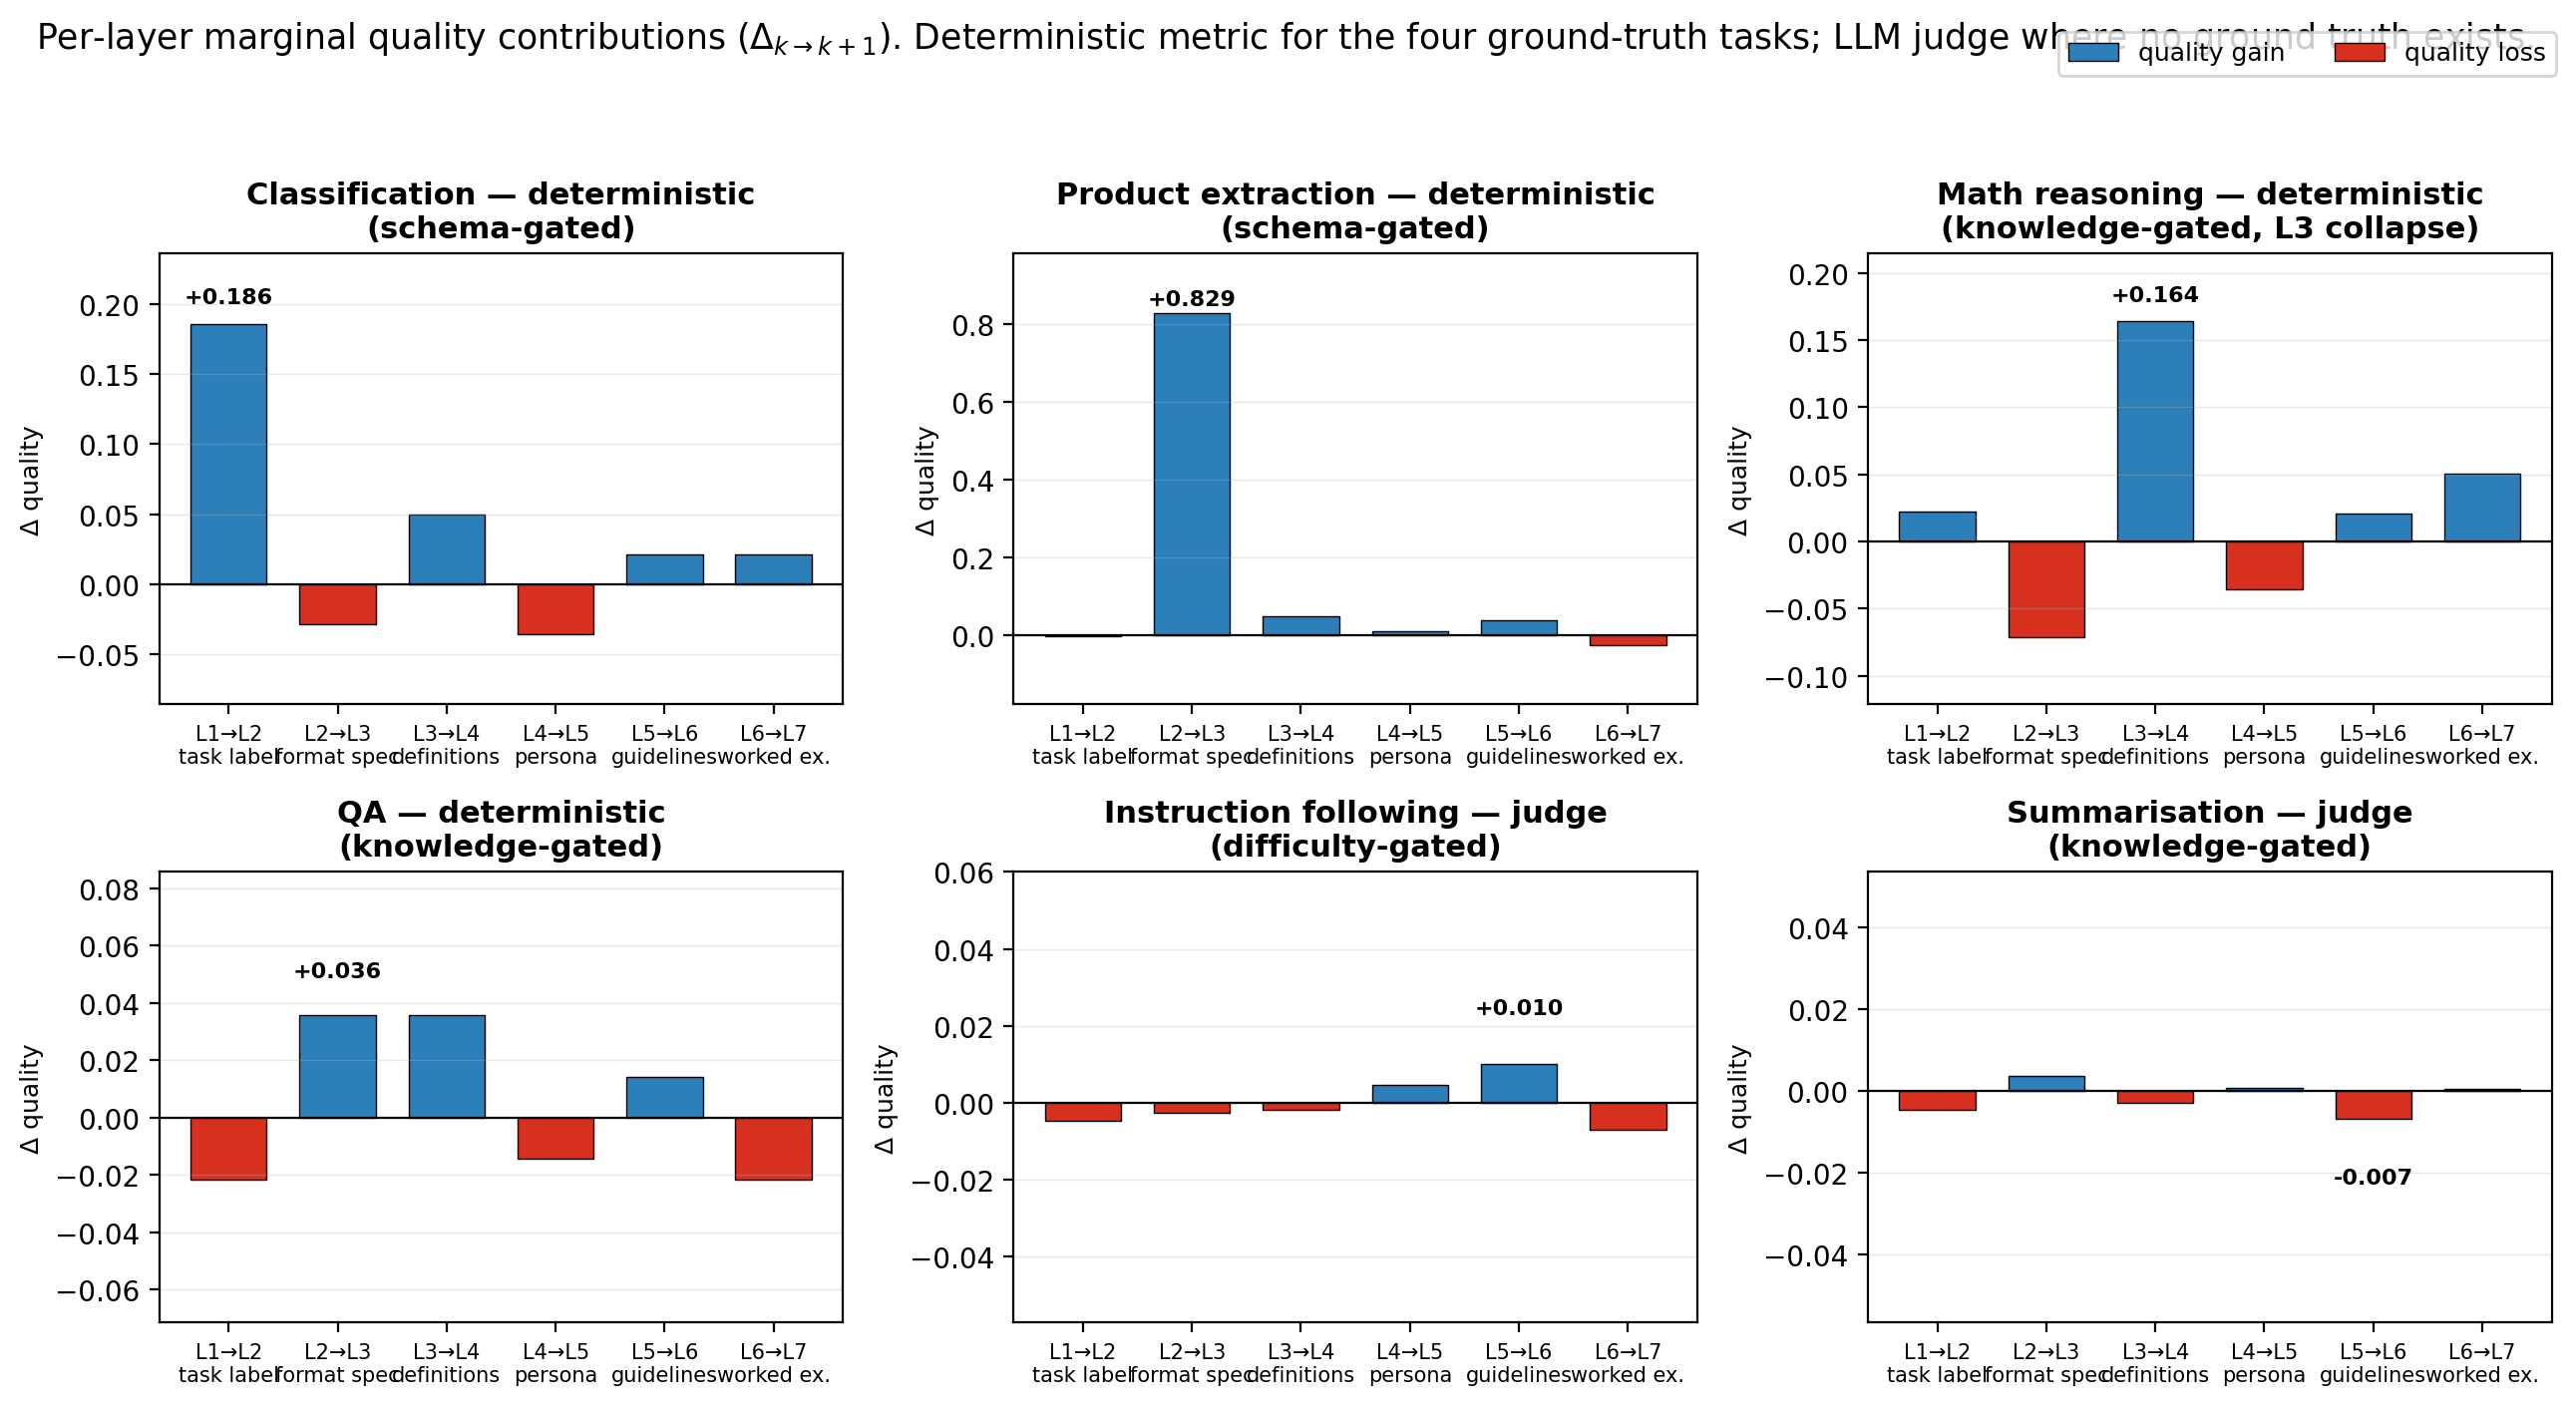
\includegraphics[width=\linewidth]{figures/fig2_marginal_contributions.png}
  \caption{Per-layer marginal quality contributions ($\Delta_{k \to k+1}$)
    averaged across models. The four ground-truth tasks use the
    \textbf{deterministic} metric (our primary measure); the two tasks without
    clean ground truth (instruction following, summarisation) use the LLM judge.
    Classification gain concentrates at L1$\to$L2 (task label, 87\%); product
    extraction concentrates at L2$\to$L3 (JSON format, 92\%); QA is flat; math
    reasoning shows a sharp L2$\to$L3 dip from suppressing chain-of-thought,
    recovered at L4. The judge-scored counterpart for the four ground-truth
    tasks, which spuriously spreads product-extraction gain onto the L6$\to$L7
    worked example, is in Appendix~\ref{app:judge-marginal}.}
  \label{fig:marginal}
\end{figure}

\paragraph{Classification (schema-gated).}
On the deterministic metric, adding the task label (L1$\to$L2) contributes
$+0.186$ quality, \textbf{87\%} of the total L1$\to$L7 gain ($+0.214$).
The LLM judge, which gives partial credit to L1's verbose-but-correct answers,
compresses this to a $+0.073$ jump (49\% of its smaller total); the ground-truth
metric exposes the full step. Subsequent layers add little, and the persona
layer is slightly harmful. A single well-chosen instruction, the label space,
captures the benefit. Output length drops from 85.1 tokens at L1 (verbose
explanation) to 2.1 tokens at L3+ (just the label) as the format takes effect:
once the model learns the output schema, further elaboration adds nothing.

\paragraph{Product extraction (schema-gated).}
The metric choice is decisive here. Under the LLM judge, gain appears spread
between the field-name layer (L1$\to$L2, $+0.054$) and the worked example
(L6$\to$L7, $+0.067$), suggesting a distributed profile. On the deterministic
field-matching metric, the picture collapses to a single layer: the
\textbf{JSON format specification at L3} accounts for $+0.829$ of the $+0.903$
total gain, or \textbf{92\%}. Quality is $\approx 0.00$ at L1--L2 and above
$0.83$ at L3. The worked example adds essentially nothing on ground truth
($-0.02$ at L6$\to$L7); the judge had rewarded it cosmetically. Product
extraction is therefore concentrated, not distributed, and we treat the judge's
distributed reading as a documented evaluation artefact
(Section~\ref{sec:result-judge}).

\paragraph{Math reasoning (non-monotonic).}
Math is knowledge-gated overall, but L3 (``Give only the final numerical
answer'') causes a sharp non-monotonic dip by suppressing chain-of-thought
reasoning~\citep{wei2022cot}. The size of the dip depends on the metric, and the
gap is itself informative: on the LLM judges the collapse is dramatic
(L2$=0.967 \to$ L3$=0.601$, $\Delta=-0.366$, across all seven models and both
judges), because the judge penalises the missing reasoning; on exact
final-answer matching it is milder (L2$=0.81 \to$ L3$=0.74$, $\Delta=-0.071$),
because models often still reach the correct number without showing work. Either
way the effect is real and recovers at L4 when step-by-step reasoning is
restored. The practical point is robust to metric choice: instructing a model to
skip its reasoning is actively harmful, never merely neutral. Excluding L3, the
trajectory is flat, consistent with ceiling-at-L1.

\paragraph{QA (insensitive).}
Total marginal gain is essentially zero (L1$\to$L7 $\Delta = -0.035$). Every
layer beyond bare input either adds nothing or slightly hurts; models already
score 0.89--0.95 at L1.

\paragraph{Three mechanism-anchored classes.}
On the deterministic metric, the three structured tasks share one profile: gain
concentrates at the single schema-resolving layer (classification 87\% at L2;
product extraction 92\% at L3; NER 95\% at L3,
Section~\ref{sec:result-holdout}). We call this class \textbf{schema-gated}. The
remaining tasks split by \emph{why} the schema layer does not dominate.
Instruction following is \textbf{difficulty-gated}: near-flat on easy
single-constraint examples but rising $6.6\times$ on hard multi-constraint ones
(Section~\ref{sec:result-nosat}). QA, math, and summarisation are
\textbf{knowledge-gated}: already at ceiling from the bare input, because the
answer depends on the model's parametric knowledge, not on prompt form. Each
class is anchored to an identifiable mechanism (schema resolution, constraint
difficulty, parametric sufficiency) rather than to the shape of an aggregate
curve, and the held-out NER task confirms the schema-gated class predictively.
Curve fitting alone under-detects step-shaped concentration (classification:
2/7 significant despite an 87\% L2 jump); marginal-contribution analysis on
ground truth recovers it, which is why we report both.

\subsection{Controls: Information Content, Not Token Count}
\label{sec:result-controls}

Two controls separate information content from raw token count: a randomised
layer-ordering ablation and an irrelevant-padding experiment. They converge on
the same conclusion: tokens do not buy quality, information does.

\paragraph{Randomised ordering.}
If saturation is driven by token count, shuffling the layer order should not
move the quality-versus-token curve; if it is driven by information content, the
saturation \emph{point} should shift with ordering while the saturation
\emph{shape} persists. Table~\ref{tab:ablation} summarises the product-extraction
results. The three most prompt-sensitive models (qwen3-32b, llama-3.1-8b,
llama-3.3-70b) show robust saturation across orderings: 13/15 fits are
significant, with saturation points clustering at 65--140 tokens regardless of
which layers come first. The more prompt-insensitive models (gemini-flash,
claude-haiku) show flatter curves with fewer significant fits (1/10), consistent
with reaching high quality from minimal prompting.

\begin{table}[t]
\centering
\caption{Randomised ablation results for product extraction.
  Mean $\pm$ standard deviation of saturation points across 5 random
  permutations.
  Significant fits: number of permutations producing $p < 0.05$.}
\label{tab:ablation}
\small
\begin{tabular}{lcrr}
\toprule
Model & $T^*$ Mean $\pm$ Std (tokens) & Range & Sig.\ fits \\
\midrule
qwen3-32b     & $95 \pm 26$  & [65, 134]  & 5/5 \\
llama-3.1-8b  & $110 \pm 24$ & [84, 140]  & 4/5 \\
llama-3.3-70b & $110 \pm 22$ & [80, 131]  & 4/5 \\
gemini-flash  & $57 \pm 17$  & [49, 91]   & 1/5 \\
claude-haiku  & $58 \pm 0$   & [58, 58]   & 0/5 \\
\bottomrule
\end{tabular}
\end{table}

The ablation is judge-scored; on that metric it places saturation at 65--140
tokens, below the fixed-ordering judge estimates for the same models (92--378
tokens). This shift is exactly what the information-content hypothesis predicts:
in the fixed ordering the schema-resolving layer sits at a fixed position, so
quality stays low until that token count is reached; when ordering is
randomised, the high-value layer can appear early and the curve bends sooner.
The shape survives reordering while the token count tracks the schema layer's
position, and raw token count cannot explain a threshold that relocates when
only the ordering changes. Classification shows only 2/25 significant fits in
the ablation, consistent with its step-shaped profile: once the task label
appears at any position, quality jumps and the curve is flat thereafter. This is
a method-shape mismatch (curve fitting under-detects steps), not an absence of
prompt sensitivity, the same reason the deterministic classification fits are
2/7 despite an 87\% L2 jump.

\paragraph{Irrelevant padding.}
The padding experiment tests the token-count null directly: do tokens themselves
buy quality? Across 1,470 runs, quality with irrelevant padding remained flat or
declined (mean L1$\to$L7 $\Delta = -0.074$ for classification, $-0.013$ for
product extraction). Only 1 of 26 conditions showed a significant positive trend
(Spearman $p < 0.05$), a near-ceiling case (claude-haiku classification,
$\Delta = +0.03$, from 0.97 to 1.00) consistent with chance at 26 tests; three
of 26 significant trends were negative, meaning padding slightly hurt quality.
Real prompt content over the same token range produced clear gains: $+0.10$ for
classification and $+0.16$ for product extraction. Real content exceeds padding
for 9 of 10 model--task pairs (full per-model comparison in the supplementary
material), with the largest gaps in llama-3.1-8b classification ($+0.190$ vs.\
$-0.161$) and qwen3-32b product extraction ($+0.220$ vs.\ $-0.038$).

\subsection{Why QA and Math Do Not Saturate}
\label{sec:result-nosat}

Two questions remain for the flat tasks. First, are they at a quality ceiling
that hides latent sensitivity? Second, does ``insensitive'' simply mean ``easy''?
Stratification answers the first and a hard-example stress test settles the
second.

\paragraph{Ceiling stratification.}
Stratifying by Level-1 quality (a $0.85$ threshold) reveals a ceiling effect:
across models, 16--20 of 20 QA examples already score above 0.85 at L1, leaving
too few below-ceiling examples for reliable curve fitting. The above-ceiling
subset shows flat-to-declining quality (gemini-flash: L1$=0.94$, L7$=0.91$; mean
$\Delta = -0.035$), consistent with extra layers adding noise to already-correct
responses. Math shows the same pattern (17--19 of 20 above 0.85 at L1) with the
L3 non-monotonicity superimposed. Classification and product extraction, by
contrast, start below ceiling because the prompt must communicate format
requirements the model cannot infer from the input alone. Restricting to
below-ceiling examples reveals latent sensitivity (classification, 32.9\% of
pairs, gains $+0.316$; product extraction, 92.8\% below ceiling, gains $+0.167$;
math, 9.4\% below ceiling, gains $+0.204$), but this subset is selected on low
L1 quality, so part of the gain is regression to the mean. We therefore do not
rest any claim on it, and turn to independently difficult examples.

\paragraph{Hard examples.}
We draw genuinely hard items from public benchmarks: multi-step GSM8K
problems~\citep{cobbe2021gsm8k} (5--8 steps) for math, multi-hop HotpotQA
questions~\citep{yang2018hotpotqa} for QA, and multi-constraint instructions
(3--5 simultaneous constraints) for instruction following, with 20 examples
each across three models (1,260 runs).
QA is knowledge-gated, not merely easy: hard examples push L1 quality well below
ceiling ($q_{\text{L1}} = 0.578$ vs.\ $0.918$ on the original set), yet the
L1$\to$L7 gain stays near zero ($\Delta = +0.021$). Elaboration does not help
even when the model starts far from correct, because the bottleneck is the
model's parametric knowledge of the answer, not the form of the prompt. This is
the cleanest possible answer to the ceiling-artefact concern.
Instruction following behaves oppositely: hard, multi-constraint instructions
amplify sensitivity \textbf{6.6$\times$} ($\Delta = +0.087$ vs.\ $+0.013$ on the
originals), with the largest gains on llama-3.3-70b ($+0.147$) and gemini-flash
($+0.108$). The definition and guideline layers that single-constraint examples
cannot distinguish from noise become load-bearing once enough constraints must
be satisfied at once, so its position depends on example difficulty rather than
on a fixed schema layer.
Math sits between: gemini-flash drops to $q_{\text{L1}} = 0.225$ on hard GSM8K
and gains $+0.112$, while llama-3.3-70b stays at ceiling
($q_{\text{L1}} = 0.988$, $\Delta = -0.003$). Math is knowledge-gated when the
model can already solve the problem and edges toward difficulty-gated when it
cannot, a model$\times$difficulty interaction. Together these results justify
the three-class account: the same manipulation leaves QA flat (knowledge-gated)
while making instruction following sharply responsive (difficulty-gated), so the
two cannot be the same ``insensitive'' category.

\subsection{Model Capability Modulates Saturation}
\label{sec:result-capability}

Within classification, API-tier models (gemini-flash, gpt-4o-mini) saturate at
lower token counts ($\approx$42--50 tokens) than the 70B Llama model (64
tokens): models that can infer the task from less context reach the plateau
sooner. Within product extraction the pattern reverses: API-tier models saturate
\emph{later} (claude-haiku at 536 tokens vs.\ llama-3.3-70b at 92 tokens) but
reach \emph{higher} asymptotic quality. For tasks where the model must
\emph{infer} what to do (classification), more capable models need less prompt;
for tasks where the prompt provides \emph{actionable format specifications}
(extraction), more capable models leverage more of them, continuing to improve
where smaller models plateau early at lower quality.

\paragraph{Sub-8B extension.}
To test whether this trend extends below the 8B floor, we evaluate Llama-3.2-1B
on classification and product extraction (332 runs). The 1B model starts
significantly lower at L1 (classification: $q=0.467$ vs.\ 0.780 for 8B) and
gains $1.58\times$ more from elaboration (L1$\to$L7 $\Delta = +0.300$ vs.\
$+0.190$). For product extraction it \emph{completely fails} at L1--L2
($q=0.000$), then jumps to $q=0.776$ at L3 when format specifications appear.
The capability-modulated trend therefore holds monotonically from 1B to 70B+:
smaller models are more prompt-sensitive, requiring more elaboration and
benefiting more from it, but saturate at lower asymptotic quality.

\subsection{Held-Out Task Confirms the Schema-Gating Mechanism}
\label{sec:result-holdout}

A taxonomy is only useful if it predicts the behaviour of tasks it was not built
from. We selected Named Entity Recognition (NER) as a held-out task and
registered a specific prediction before running it, then evaluated it on five
models scored on per-type F1 (deterministic ground truth).

\paragraph{Prediction.}
NER produces structured output (JSON lists of typed entities) the model cannot
infer from a bare sentence. Under the schema-gating account it should be
\textbf{schema-gated}: a single format-specification layer should unlock the
task and capture almost all of the gain, with later layers (definitions,
persona, guidelines, worked example) adding little.

\paragraph{Result: confirmed.}
Four of five models produce significant saturating curves ($p < 0.05$; $R^2 >
0.98$ for all four). The marginal-contribution profile matches the prediction
exactly: NER is \textbf{concentrated at L3} (the JSON format specification),
which accounts for $+0.750$ quality, \textbf{95\%} of the total L1$\to$L7 gain
($+0.788$). Four of five models score exactly $q = 0.000$ at L1--L2 (complete
failure to produce parseable output), then jump to $q > 0.90$ at L3, the same
step, at the same layer, as product extraction.

\paragraph{Why this matters.}
The held-out task elevates schema-gating from a post-hoc description to a
mechanism with out-of-sample predictive power: we predicted both the class
(schema-gated) and the specific layer (L3 format) for a task the framework had
never seen, and ground truth confirmed both. It also pins down the mechanism
precisely. The decisive ingredient is not ``structured output'' in general but
resolution of the \emph{output schema}, the layer that tells the model what
shape the answer must take. A secondary observation: product extraction's four
heterogeneous fields (name, price, brand, category) leave slightly more for
later layers than NER's three homogeneous entity lists, so schema
\emph{complexity} modulates how sharply the step concentrates, but in both cases
the format layer dominates.

\subsection{Evaluator Reliability: Judge vs.\ Ground Truth}
\label{sec:result-judge}

We deliberately avoid resting conclusions on a single LLM evaluator, and verify
this from two directions: an independent second judge, and a head-to-head
comparison of the judge against deterministic ground truth.

\paragraph{Second judge.}
We re-evaluated all 3,915 main-study judge responses with an independent second
judge (gemini-2.0-flash) using the identical rubric. Agreement is strong where
the judge carries variance: classification ($r = 0.835$, MAE$= 0.044$) and math
reasoning ($r = 0.859$, MAE$= 0.033$). For QA and product extraction, Pearson
$r$ is low ($0.287$ and $0.247$), but this reflects ceiling compression rather
than pattern disagreement: the gemini judge assigns scores $> 0.9$ to 98.8\% of
QA responses and 88.7\% of product-extraction responses, leaving almost no
variance to correlate. Both judges agree on the L1$\to$L7 direction for 5/7
models on classification and 4/7 on product extraction; the 3
product-extraction non-agreements involve gemini deltas of $\leq 0.003$.

\paragraph{Judge vs.\ ground truth.}
The judge is least trustworthy precisely on product extraction (inter-judge
$r = 0.247$), the task with the strongest saturation, so the natural worry is
that the saturation signal is a judge artefact. We score all 3,915 ground-truth
responses with deterministic evaluators (exact-match for classification and
math, field-matching for product extraction, ROUGE-1 containment for QA) and
compare in Table~\ref{tab:heuristic-agreement}.

\begin{table}[t]
\centering
\caption{Judge vs.\ heuristic agreement. Per-record Pearson~$r$ and MAE
  measure point-level agreement; curve-shape~$r$ measures whether the
  7-level quality trajectory agrees; direction agreement counts how many
  of 7 models show the same L1$\to$L7 sign.}
\label{tab:heuristic-agreement}
\small
\begin{tabular}{lrrrrr}
\toprule
Task & per-record $r$ & MAE & curve-shape $r$ & L1$\to$L7 dir.\ & heuristic sig. \\
\midrule
Classification      & 0.926 & 0.069 & 0.839 & 6/7 & 2/7 \\
Product extraction  & 0.415 & 0.300 & 0.660 & 7/7 & 7/7 \\
QA                  & 0.178 & 0.127 & 0.098 & 0/7 & 0/7 \\
Math reasoning      & 0.539 & 0.144 & 0.525 & 5/7 & 1/7 \\
\bottomrule
\end{tabular}
\end{table}

The comparison resolves the worry decisively. Product extraction, the task the
judge scored least reliably, shows \textbf{7/7 significant} saturation fits under
the deterministic metric versus 3/7 under the judge, with 7/7 L1$\to$L7
direction agreement. The signal is stronger and cleaner on objective field
matching, so it cannot be an artefact of judge noise. The judge's lower
reliability here stems from ceiling compression, not random error: it assigns
prose responses partial credit and caps the variance, which both inflates low
levels (masking the L3 step) and spreads apparent gain onto the worked example.
Ground truth is binary about format compliance and exposes the true step.
The metric also relocates \emph{where} the gain sits. Under the judge,
product-extraction gain looked spread across L1$\to$L2 and L6$\to$L7; under
ground truth, \textbf{92\%} of the gain is the L3 format specification and the
worked example contributes nothing. For classification, the task label
(L1$\to$L2) carries \textbf{87\%} of the ground-truth gain ($+0.186$ of
$+0.214$), and the held-out NER task shows the same L3 concentration (95\%),
confirming the mechanism is schema resolution, not example demonstration. QA is
flat under both metrics (0/7 significant), independently confirming it is
knowledge-gated. This is why we adopt the deterministic metric as primary: where
the two disagree, the disagreement is itself diagnostic, and ground truth is the
arbiter.

\subsection{Robustness: Threshold, Scale, and Sampling}
\label{sec:result-robust}

Three checks confirm that the schema-gated findings are not artefacts of the
saturation threshold, the dataset size, or the per-condition sample.

\paragraph{Threshold sensitivity.}
For classification, saturation points are stable across threshold choices: the
median 90\%-to-95\% shift across all 7 models is 3 tokens, and 6 of 7 models
shift by fewer than 11 tokens. One outlier, qwen3-32b, follows a logarithmic
rather than sigmoid trajectory, producing a 95-token shift; it uniquely benefits
from the guidelines layer (L6), suggesting it integrates detailed instructions
more gradually. Its threshold-free knee estimate (42 tokens) falls close to the
other models', confirming similar saturation onset despite the different curve
shape.

\paragraph{Larger-dataset replication.}
We replicate the two endpoint tasks on 200 examples from standard benchmarks:
classification on SST-2 and QA on SQuAD, with identical prompt templates.
Classification again shows a clear sigmoid with saturation at $\approx$64
tokens, consistent with the curated main study and confirming the schema-gated
pattern on a standard dataset at $10\times$ the sample size. QA shows no
significant prompt-length effect, reinforcing its knowledge-gated status. The
positive (schema-gated) and negative (knowledge-gated) poles both hold at scale
on public data, bounding the intermediate tasks.

\paragraph{Sampling stability.}
A common concern with $n=20$ per level is that single-run quality conflates the
prompt effect with sampling noise. We test this by repeating the full experiment
(3 schema/difficulty-critical tasks $\times$ 7 levels $\times$ 20 examples) two
additional times at temperature zero on three models (llama-3.1-8b,
llama-3.3-70b, and gemini-flash), for 2,520 extra runs. The key quantity is the
\emph{effect-to-noise ratio}: the L1$\to$L7 quality delta divided by the
across-run standard error of the level means. These ratios are large,
\textbf{20--139 for classification and 29--64 for product extraction across the
three models}, meaning the prompt effect exceeds run-to-run noise by one to two
orders of magnitude. The per-run deltas bear this out: classification
$\Delta = +0.190, +0.235, +0.245$ (llama-3.1-8b, std $= 0.024$), product
extraction $\Delta = +0.097, +0.133, +0.120$ (std $= 0.015$), while instruction
following on llama-3.1-8b is the sole near-noise case ($\Delta = +0.062, -0.005,
+0.000$, std $= 0.031$, ratio $\approx 2$), exactly the difficulty-gated task
that is flat on easy examples. L7 quality is especially stable (classification:
0.970 across all three runs), with most variance at L1 where the bare input
gives least guidance. The small per-condition sample is thus not a source of
fragility for the schema-gated effects: they reproduce run to run. Gemini-flash
repeated runs used gemini-2.5-flash, as gemini-2.0-flash was deprecated between
study phases; runs 1 and 2 are near-identical (classification $\Delta = +0.345$
vs.\ $+0.347$), confirming temperature-zero determinism, and the direction of
all effects is preserved across both model versions.
